\input ../../SlidePreamble
\input ../../preamble

\begin{document}

{\Huge
  \centerline{\bf TTIC 31230,  Fundamentals of Deep Learning}
  \vfill
  \centerline{David McAllester, Autumn 2021}
  \vfill
  \centerline{\bf 2021 Developments}

\vfill
\vfill

\slide{Wav2vec 2.0, June 2020, Facebook}

\vfill
Trained on 53k hours of unlabeled audio (no text) they convert speech to a sequence of discrete quantized vectors they call ``pseudo-text units''.

\vfill
By training on only one hour of human-transcribed audio, and using the Wav2vec transcription into pseudo-text, the outperform the previous state of the
in word error rate for 100 hours of human-transcribed text.


\slide{GLSM, February 2021, Facebook}

Generative Spoken Language Model (GLSM)



\vfill
They then train a generative model of the sequences of pseudo-text units learned from unlabeled audio.


\vfill
This model can continue speech from a speech prompt in much the same way that GPT-3 continues text from a text prompt.

\vfill
Semantic and grammatical structure in a ``unit language model'' is recovered
from speech alone.


\slide{CLIP, January 2021, OpenAI}

CLIP: Contrastive Language-Image Pre-training.

\vfill
Trained on images and associated text (such as image captions or hypertext links to images).

\vfill
The model computes a probability of text given image.

\vfill
It is then used for zero-shot image classification on various datasets.

\vfill
One can classify an image by comparing the probabilities that the model assigns to ``prompts''.  There is a prompt for each class.

\slide{Zero-Shot Image Classification}

\centerline{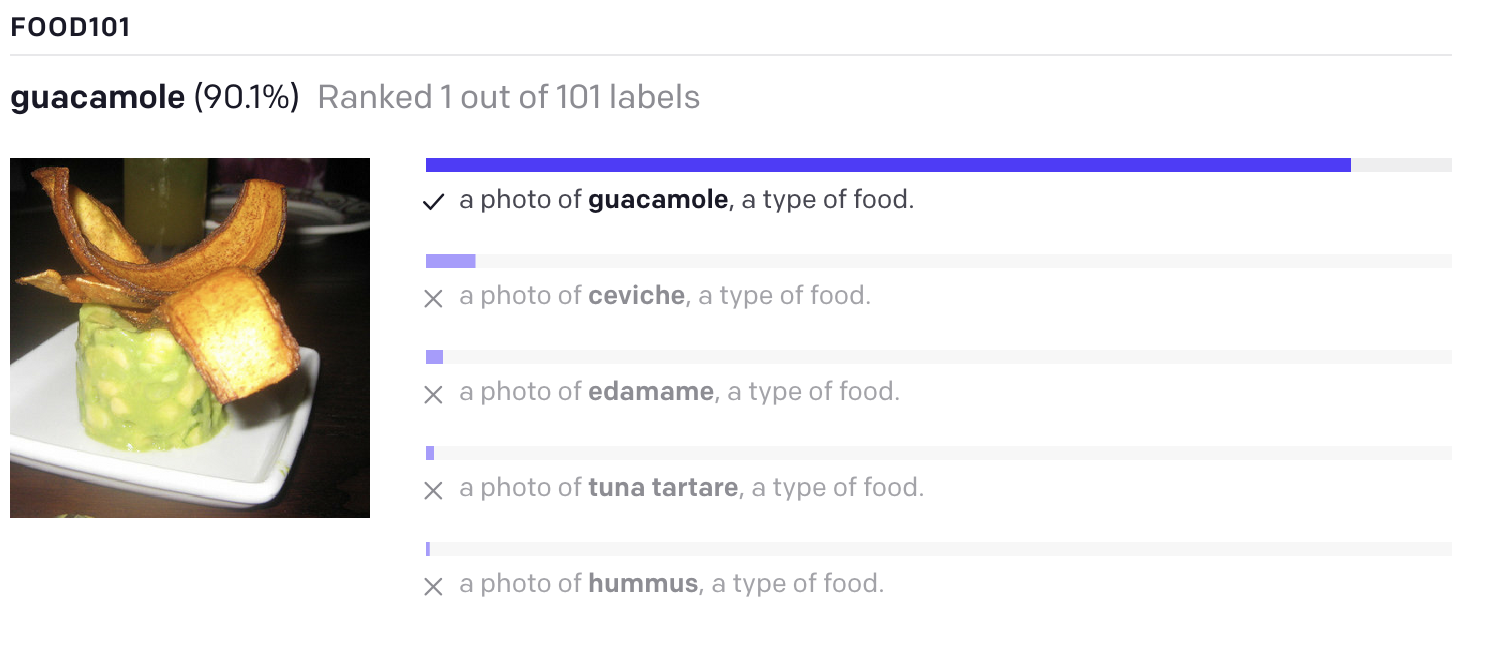
\includegraphics[width = 7in]{\images/CLIP0}}

\slide{Zero-Shot Image Classification}

\centerline{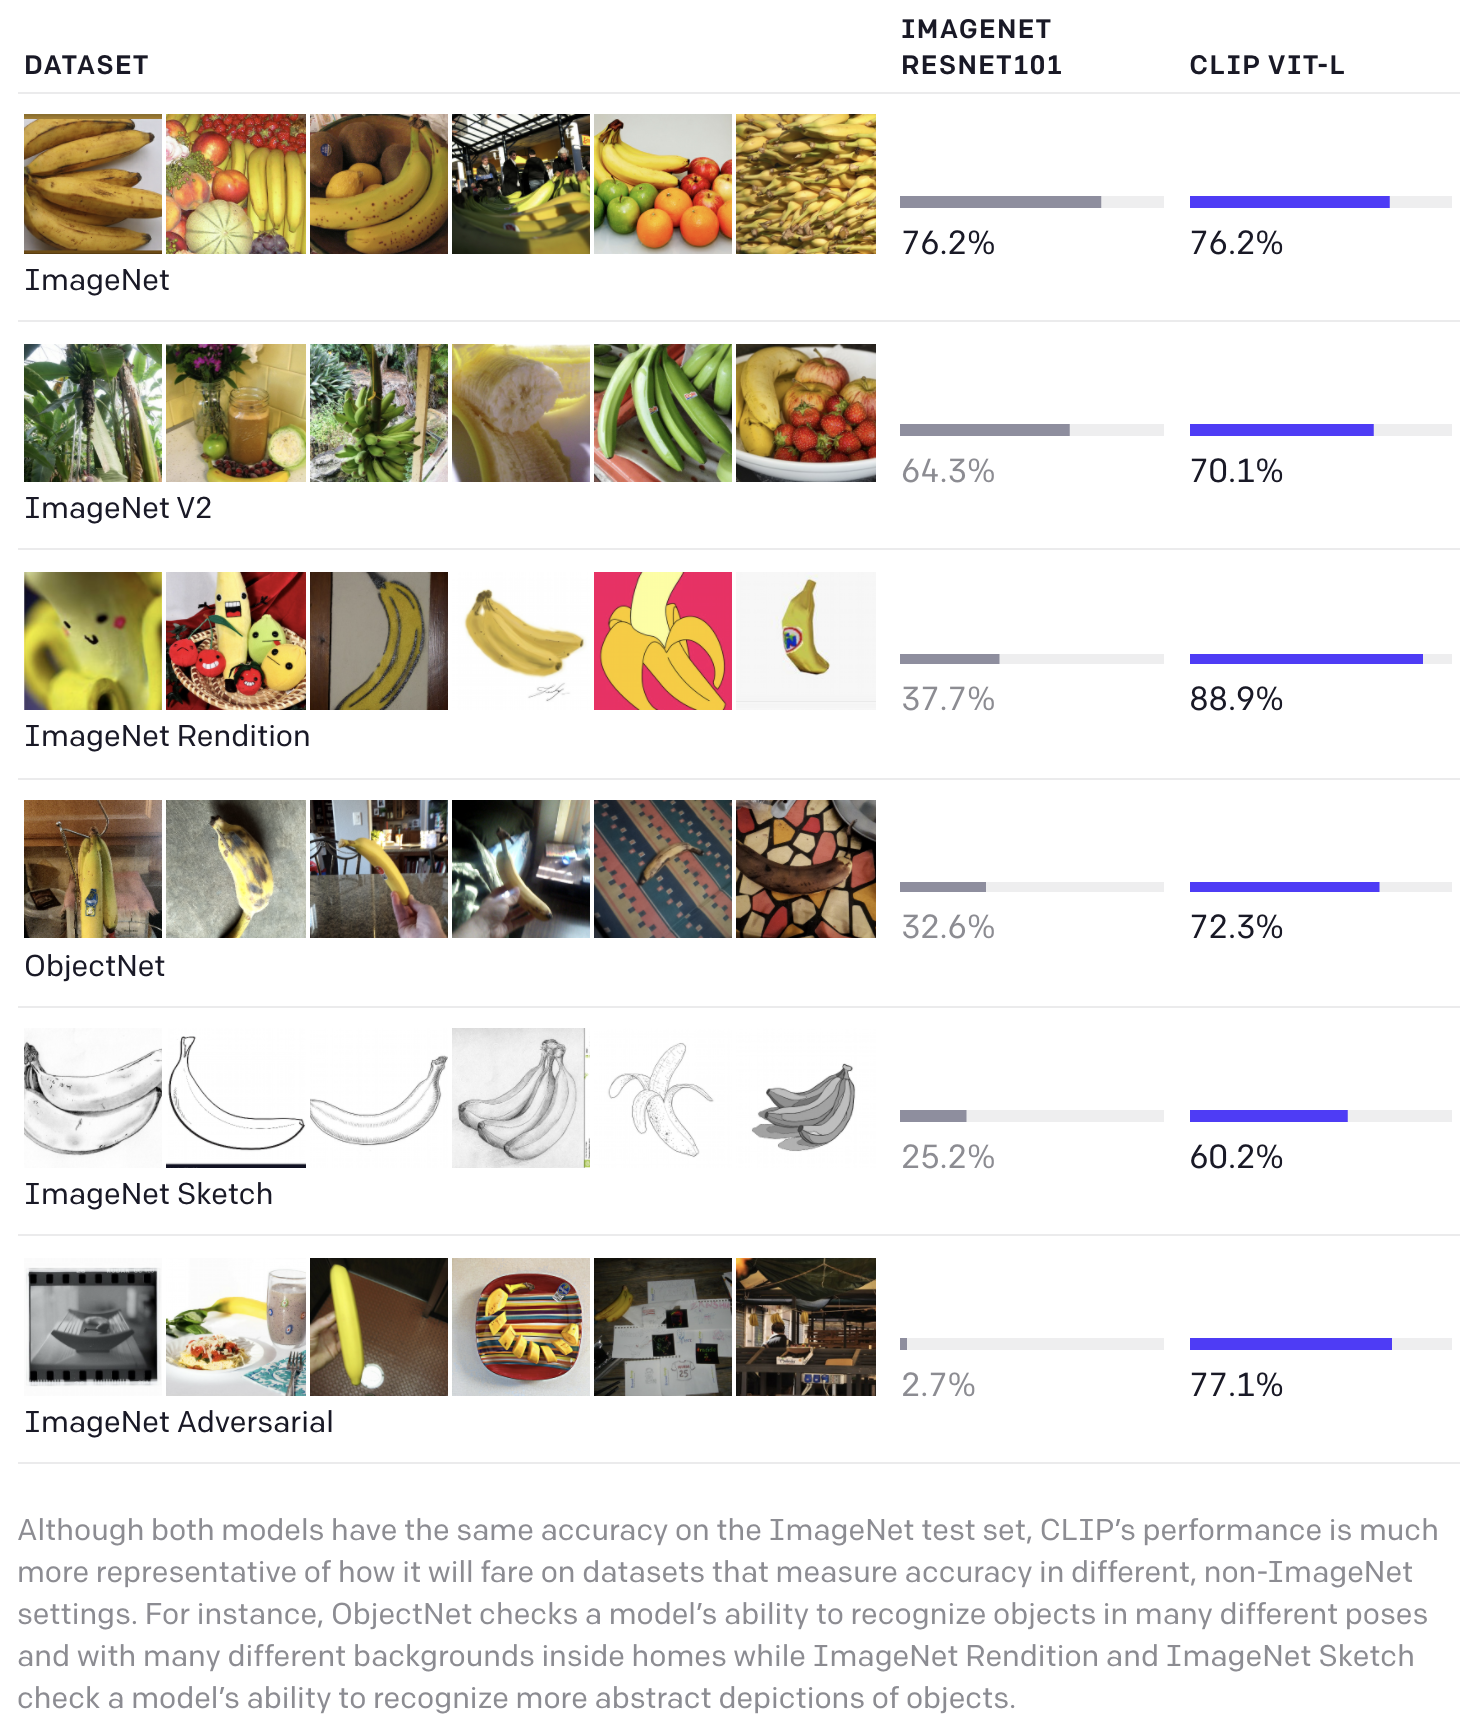
\includegraphics[height= 5in]{\images/CLIP1}}

\slide{DALL$\cdot$E, January 2021, OpenAI}

The name DALL$\cdot$E is simply some kind of homage to the painter Dali and the Disney character WALL$\cdot$E.

\vfill
Like CLIP, DALL$\cdot$E is trained on images paired with text (pressumably the same data as CLIP).  DALL$\cdot$E and CLIP were announced by OpenAI on the same day, although they are different systems.

\vfill
Given text, DALL$\cdot$E generates an image.


\slide{Zero-Shot Image Rendering from Language}

\centerline{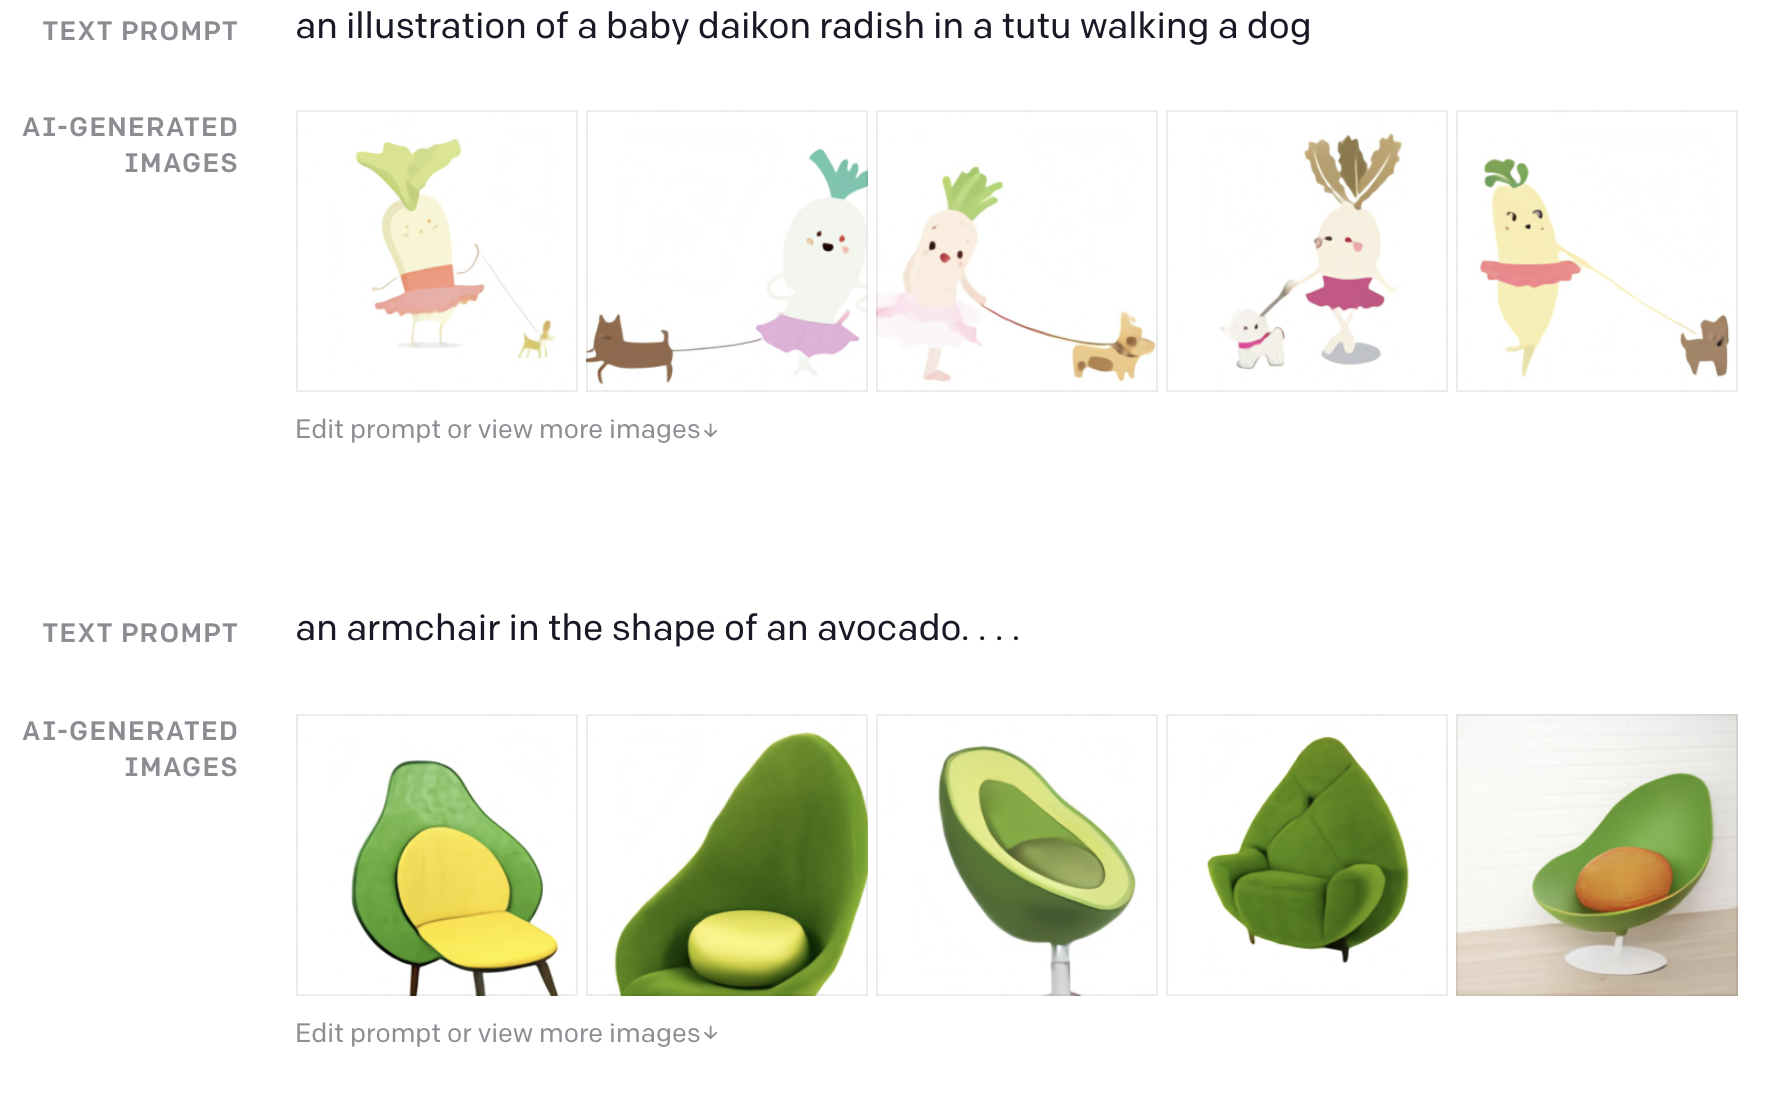
\includegraphics[height= 5in]{\images/DALLE1}}

\slide{Codex, July 2021, OpenAI}

This is a language model trained on code, including comments, from public repositories.

\vfill
Starting from an English prompt Codex continues with code --- a form of automatic programming.

\vfill
There is a published version (58 authors) and a production version that powers {\bf GitHub Copilot}.

\vfill
Copilot may supplant Stack Overflow for finding out how to do x in language y.

\vfill
It also seems possible that some version Codex will replace, or at least augment, speech assistants such as Siri.

\slideplain{Application Advancements vs. Architecture Advancements}

Advancements in the general principles of learning are having applications over very diverse applications.

\vfill
When considering Moore's law of AI it seems worth distinguishing architectural advancements (new general learning methods)
from new applications of established architectures.

\vfill
This course will focus on general, architectural, ideas and how they have advanced in recent years.

\slideplain{END}

}
\end{document}
